\chapter{Results and Discussion}
\label{ch:05_Results_Discussion}
\section{Parameter Study} \label{section:ParameterStudy}
\begin{figure} [H]
	\begin{subfigure}{0.45\columnwidth}%
		\centering
		\begin{tikzpicture}
	\begin{axis}[
								xmin=0,
								xmax=2.5,
								ymin=40000000,
								ymax=60000000,
								width=8cm,
								xtick pos=left,
								xlabel={normalized viscosity $\frac{\nu}{\nu _A}/ - \ \longrightarrow$},
								ylabel={pressure drop $\frac{\Delta P}{L}\ /\ \si{\pascal\per\metre} \longrightarrow$},
								clip=false,
								legend cell align=left,
								legend style={draw=none, font=\small, column sep=0.3em, fill=none, anchor=north west, at={(rel axis cs: 0.05,1)}}
							]
			\addplot[only marks, mark options={color=TUMBlauDunkel, mark=diamond*, scale=1.4}] table[x index = 0,y index = 1]{Figures/pressure/data/FluidViscosity_B1.txt}; \addlegendentry{$\nu/\nu_A = 0.2$ (B1)}
			
			\addplot[only marks, mark options={color=TUMBlauHell, mark=diamond*, scale=1.4}] table[x index = 0,y index = 1]{Figures/pressure/data/FluidViscosity_B2.txt}; \addlegendentry{$\nu/\nu_A = 0.04$ (B2)}
			
			\addplot[only marks, mark options={color=TUMOrange, mark=x, scale=2}] table[x index = 0,y index = 1]{Figures/pressure/data/FluidViscosity_A.txt}; \addlegendentry{$\nu_A$ (A)}
			
			\addplot[only marks, mark options={color=TUMBlauAkzent1, mark=diamond*, scale=1.4}] table[x index = 0,y index = 1]{Figures/pressure/data/FluidViscosity_B3.txt}; \addlegendentry{$\nu/\nu_A = 2$ (B3)}
	\end{axis}
\end{tikzpicture}

%\addplot[only marks, mark = circle*, mark options={color=TUMBlauHell, mark=otimes*, scale=1.2}] table[x index = 0,y index = 1]{Figures/parityplotwallmodre/OriginalErgunPdropCor_wallmodre.txt}; \addlegendentry{Original Ergun}
		\subcaption{Fluid viscosity.}
				\label{fig:SPSRViscosity}
	\end{subfigure}
	\hfill
	\begin{subfigure}{0.45\columnwidth}%
		\centering
		\begin{tikzpicture}
\begin{axis}[
%xmode=log,
%ymode=log,
xmin=0,
xmax=200,
ymin=1E6,
ymax=1.5E9,
width=8cm,
xtick pos=left,
xlabel={superficial velocity $u_0 / \si{\metre\per\second} \longrightarrow$},
ylabel={pressure drop $\frac{\Delta P}{L}\ /\ \si{\pascal\per\metre} \longrightarrow$},
clip=false,
legend cell align=left,
legend style={draw=none, font=\small, column sep=0.3em, fill=none, anchor=north west, at={(rel axis cs: 0.05,1)}}
]
\addplot[only marks, mark options={color=TUMBlauDunkel, mark=triangle*, scale=1.4}] table[x index = 0,y index = 1]{Figures/pressure/data/SuperficialVelocity_C1.txt}; \addlegendentry{$N$ = 5 (C1)}

\addplot[only marks, mark options={color=TUMBlauHell, mark=triangle*, scale=1.4}] table[x index = 0,y index = 1]{Figures/pressure/data/SuperficialVelocity_C2.txt}; \addlegendentry{$N$ = 10 (C2)}

\addplot[only marks, mark options={color=TUMOrange, mark=x, scale=2}] table[x index = 0,y index = 1]{Figures/pressure/data/SuperficialVelocity_A.txt}; \addlegendentry{$N$ = 20 (A)}

\addplot[only marks, mark options={color=TUMBlauAkzent2, mark=triangle*, scale=1.4}] table[x index = 0,y index = 1]{Figures/pressure/data/SuperficialVelocity_C3.txt}; \addlegendentry{$N$ = 50 (C3)}

\addplot[only marks, mark options={color=TUMBlauAkzent1, mark=triangle*, scale=1.4}] table[x index = 0,y index = 1]{Figures/pressure/data/SuperficialVelocity_C4.txt}; \addlegendentry{$N$ = 100 (C4)}


\end{axis}
\end{tikzpicture}

%\addplot[only marks, mark = circle*, mark options={color=TUMBlauHell, mark=otimes*, scale=1.2}] table[x index = 0,y index = 1]{Figures/parityplotwallmodre/OriginalErgunPdropCor_wallmodre.txt}; \addlegendentry{Original Ergun}



%
		\subcaption{Flow velocity.}
		\label{fig:SPSRVelocity}
	\end{subfigure} \\ 
	
	\begin{subfigure}{0.45\columnwidth}%
		\centering
		\begin{tikzpicture}
\begin{axis}[
xmin=1,
xmax=1.9,
ymin=7.5E6,
ymax=1.2E8,
width=8cm,
xtick pos=left,
xlabel={diameter aspect ratio $\frac{D}{d}/ - \ \longrightarrow$},
ylabel={pressure drop $\frac{\Delta P}{L}\ /\ \si{\pascal\per\metre} \longrightarrow$},
clip=false,
legend cell align=left,
legend style={draw=none, font=\small, column sep=0.3em, fill=none, anchor=north east, at={(rel axis cs: 0.95,1)}}
]
\addplot[only marks, mark options={color=TUMBlauDunkel, mark=square*, scale=1.4}] table[x index = 0,y index = 1]{Figures/pressure/data/DiameterAspectRatio_D1.txt}; \addlegendentry{D/d = 1.125 (D1)}

\addplot[only marks, mark options={color=TUMOrange, mark=x, scale=2}] table[x index = 0,y index = 1]{Figures/pressure/data/DiameterAspectRatio_A.txt}; \addlegendentry{D/d = 1.25 (A)}

\addplot[only marks, mark options={color=TUMBlauHell, mark=square*, scale=1.4}] table[x index = 0,y index = 1]{Figures/pressure/data/DiameterAspectRatio_D2.txt}; \addlegendentry{D/d = 1.5 (D2)}

\addplot[only marks, mark options={color=TUMBlauAkzent1, mark=square*, scale=1.4}] table[x index = 0,y index = 1]{Figures/pressure/data/DiameterAspectRatio_D3.txt}; \addlegendentry{D/d = 1.75 (D3)}

\end{axis}
\end{tikzpicture}
%\addplot[only marks, mark = circle*, mark options={color=TUMBlauHell, mark=otimes*, scale=1.2}] table[x index = 0,y index = 1]{Figures/parityplotwallmodre/OriginalErgunPdropCor_wallmodre.txt}; \addlegendentry{Original Ergun}%
		\subcaption{Diameter aspect ratio.}
						\label{fig:SPSRDiameterAspect}
	\end{subfigure}
	\hfill
	\begin{subfigure}{0.45\columnwidth}%
		\centering
		%\begin{tikzpicture}
%	\begin{axis}[
%								xmin=9,
%								xmax=200,
%								ymin=2E6,
%								ymax=5E7,
%								width=8cm,
%								xtick pos=left,
%								xlabel={scaling factor $s/ - \ \longrightarrow$},
%								ylabel={pressure drop $\frac{\Delta p}{L} / Pa\:m^{-1} - \ \longrightarrow$},
%								clip=false,
%								legend cell align=left,
%								legend style={draw=none, font=\small, column sep=0.3em, fill=none, anchor=north east, at={(rel axis cs: 0.99,0.995)}}
%							]
%			\addplot[only marks, mark = triangle*, mark options={draw=TUMBlauAkzent1, fill=TUMBlauAkzent1, scale=1.8}] table[x index = 0,y index = 1]{Figures/pressure/data/ScalingFactor.txt};
%	\end{axis}
%\end{tikzpicture}

\begin{tikzpicture}
\begin{axis}[
xmin=0.5,
xmax=2,
ymin=4E7,
ymax=9E7,
width=8cm,
xtick pos=left,
xlabel={scaling factor $s/ - \ \longrightarrow$},
ylabel={pressure drop $\frac{\Delta P}{L}\ /\ \si{\pascal\per\metre} \longrightarrow$},
clip=false,
legend cell align=left,
legend style={draw=none, font=\small, column sep=0.3em, fill=none, anchor=north west, at={(rel axis cs: 0.05,1)}}
]
\addplot[only marks, mark options={color=TUMOrange, mark=x, scale=2}] table[x index = 0,y index = 1]{Figures/pressure/data/ScalingFactor_A.txt}; \addlegendentry{$s = d/d_A = 1.0$ (A)}

\addplot[only marks, mark options={color=TUMBlauDunkel, mark=otimes*, scale=1.4}] table[x index = 0,y index = 1]{Figures/pressure/data/ScalingFactor_E1.txt}; \addlegendentry{$s = d/d_A = 1.5$ (E1)}

%\addplot[only marks, mark options={color=TUMBlauHell, mark=otimes*, scale=1.4}] table[x index = 0,y index = 1]{Figures/pressure/data/ScalingFactor_E2.txt}; \addlegendentry{$s = d/d_A = 2.0$ (E2)}

\end{axis}
\end{tikzpicture}

%\addplot[only marks, mark = circle*, mark options={color=TUMBlauHell, mark=otimes*, scale=1.2}] table[x index = 0,y index = 1]{Figures/parityplotwallmodre/OriginalErgunPdropCor_wallmodre.txt}; \addlegendentry{Original Ergun}
%
		\subcaption{Geometry scaling factor.}
						\label{fig:SPSRScalingFactor}
	\end{subfigure}
	
	\caption{Influence of fluid viscosity, flow velocity, diameter aspect ratio and geometry scaling factor on pressure drop.}%
	\label{fig:SPSR-p_parameter-study}	
\end{figure}
\newpage
Fig. \ref{fig:SPSRViscosity} shows an almost linear relationship between pressure drop and fluid viscosity, with less-than-expected values for pressure drop obtained at elevated levels of normalized viscosity at $\frac{\nu}{\nu_A} = 1$ and $\frac{\nu}{\nu_A} = 2$ respectively. As mentioned previously above, the first term of the Ergun equation (cf. Eq. \ref{eqn:ErgunFromJohanna}) is mostly decisive at laminar flows and it corresponds to viscous losses. Having a wall modified Reynolds value of \num{2e3} enables turbulent simulative flow, in which the second term of the Ergun equation relating to kinetic losses becomes more dominant. Thus, a reason for the lower-than-expected values for higher normalized viscosity values of 1 and 2 thereby causing a deviation from the linear relationship observed in Fernengel et al. \cite{Fernengel2020} may be due to this dominant second term in turbulent flow, in which viscous losses are less dominant at elevated values of normalized viscosity. The observed trend can be also explained mathematically: Viscous losses represented by the dynamic viscosity term ($\eta$) is not present in the predominant second Ergun coefficient in turbulent flow.
%according to johanna, argue that the viscous losses (look at dynamic viscosity term on the first term) is NOT PRESENT in the 2nd term, hence, you may obtain a smaller-than-expected pressure drop per unit length at elevated normalised viscosity levels.
%Looking at Fig. \ref{fig:SPSR-p_velocity}, a linear relationship between pressure drop and superficial velocity similar to what was obtained in laminar flow (cf. \cite{Fernengel2020}) was observed with a logarithmic plot.

Looking at Fig. \ref{fig:SPSRVelocity}, an exponential increase in pressure drop with rising superficial velocity was observed as opposed to the linear trend discovered previously in laminar flow (cf. \cite{Fernengel2020}). This obtained results are in line with a similar simulative study performed in a two-dimensional SPSR at turbulent conditions by M\"{u}ller et al. \cite{Mueller2012}. Synonymous to M\"{u}ller et al., the slope of the pressure drop against velocity graph becomes increasingly steeper and non-linear at elevated superficial velocities and eventually displays an exponential trend. The increase in superficial velocity and hence pressure drop values with the addition of catalytic pellets in the SPSR can be explained both mathematically and theoretically. From a mathematical point of view, with reference to Eqs. \ref{eqn:u_0} and \ref{eqn:ErgunFromJohanna}: An increase in $N$ will lead to an surge in $u_0$ (ref. Eq. \ref{eqn:u_0}), which indirectly raises the $\Delta P/L$ value (ref. Eq. \ref{eqn:ErgunFromJohanna}). From a theoretical point of view, higher frictional forces between the fluid and particles will arise from increased fluid velocities thus leading to increased values of pressure drop \cite{Mueller2012}.
%Further simulations will have to be done covering an even wider range of superficial velocities to observe if this is a valid trend for turbulent flow within SPSRs.
%The pressure drop presents a measure for the flow resistance inside a channel and is a major design parameter for processes. As shown in Fig. 4a), the pressure drop increases with increasing fluid velocity due to the higher friction forces between the fluid and the particles. [Muller]. Might wanna change above to a normal vs. normal graph and explain the results citing fig 4a) from Muller cause you obtained the same trends as Muller.

The effects of varying diameter aspect ratio on pressure drop over the pellet string is depicted in Fig. \ref{fig:SPSRDiameterAspect}. Here, we observe trends similar with what was ascertained in laminar flow (cf Fernengel et al. \cite{Fernengel2020}) with respect to the reduction in pressure drop with increasing diameter aspect ratio. An increment in diameter aspect ratio (from D/d = 1.125 to 1.25) projects a greater-than threefold sharp reduction in pressure drop similar to what was observed in laminar flow. Following which, further increases in the diameter aspect ratio (from D/d = 1.25 to 1.75) leads to a less aggressive reduction in pressure drop. This pattern is predicted as there are two major flow pathways occurring in the SPSRs: one meandering around the pellets flowing from one side of the bed to the other, and the other passing the particles in a straight manner perpendicular to the plane through the pellet centres. Such flow channels adjacent to the pellet string are more prominent with increasing diameter aspect ratios, contributing to higher bed porosities for the proposed reactor geometries \cite{Fernengel2020} which mathematically leads to lower pressure drop values (referencing Eq. \ref{eqn:ErgunFromJohanna}). The aforementioned two major flow pathways are highlighted and displayed with ParaView using Case D3 as a reference model in Figs. \ref{fig:streamtracetube_p_D3} and \ref{fig:streamtracetube_p_sideview_D3}.
\begin{figure} [H]
	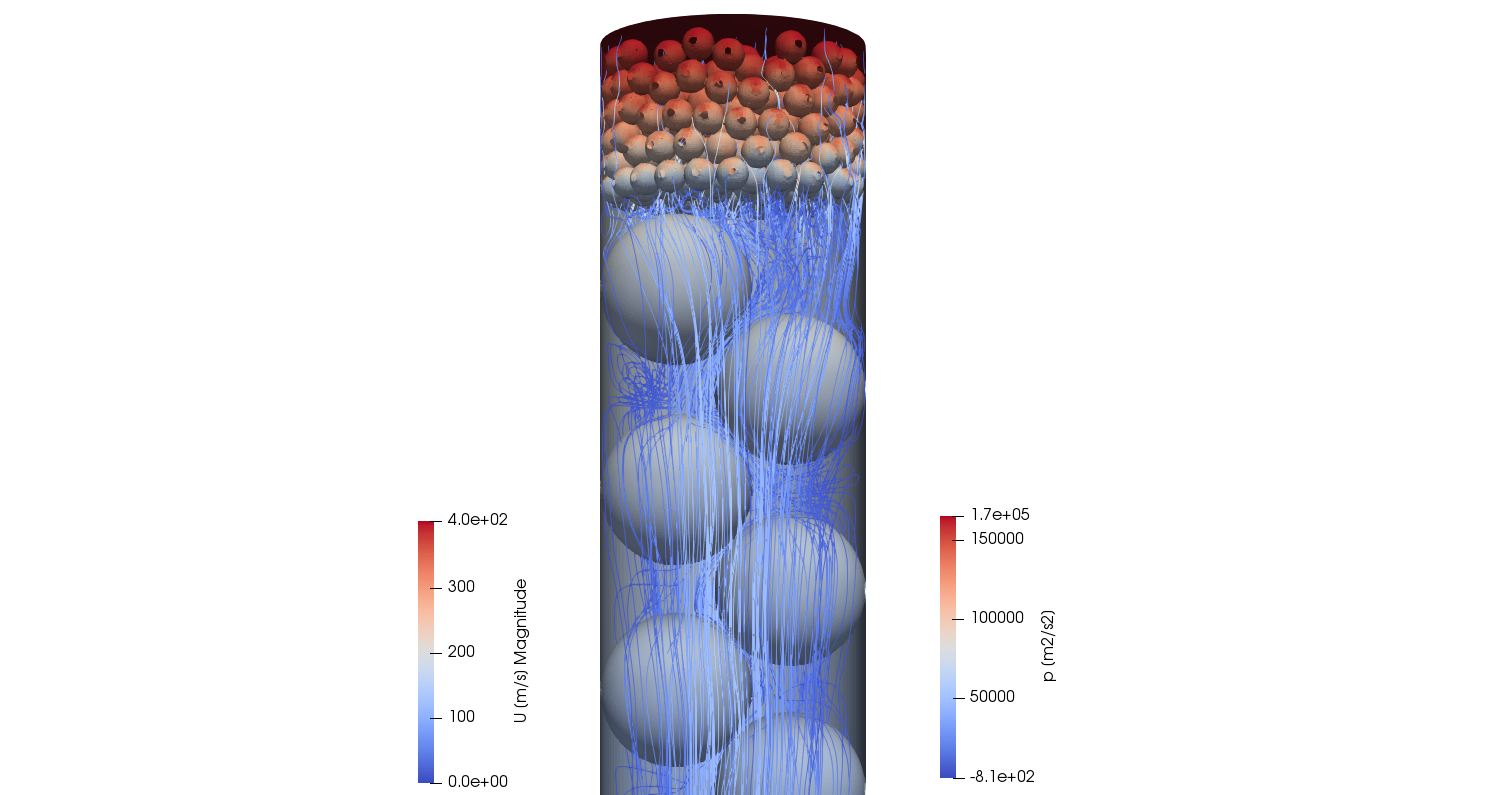
\includegraphics[width=\linewidth]{Figures/visualisation/caseD3/StreamTracer_Sphere_FrontView_withunits_CaseD3.png}
	\caption{Front view of case D3 highlighting meandering fluid flow.}
	\label{fig:streamtracetube_p_D3}

	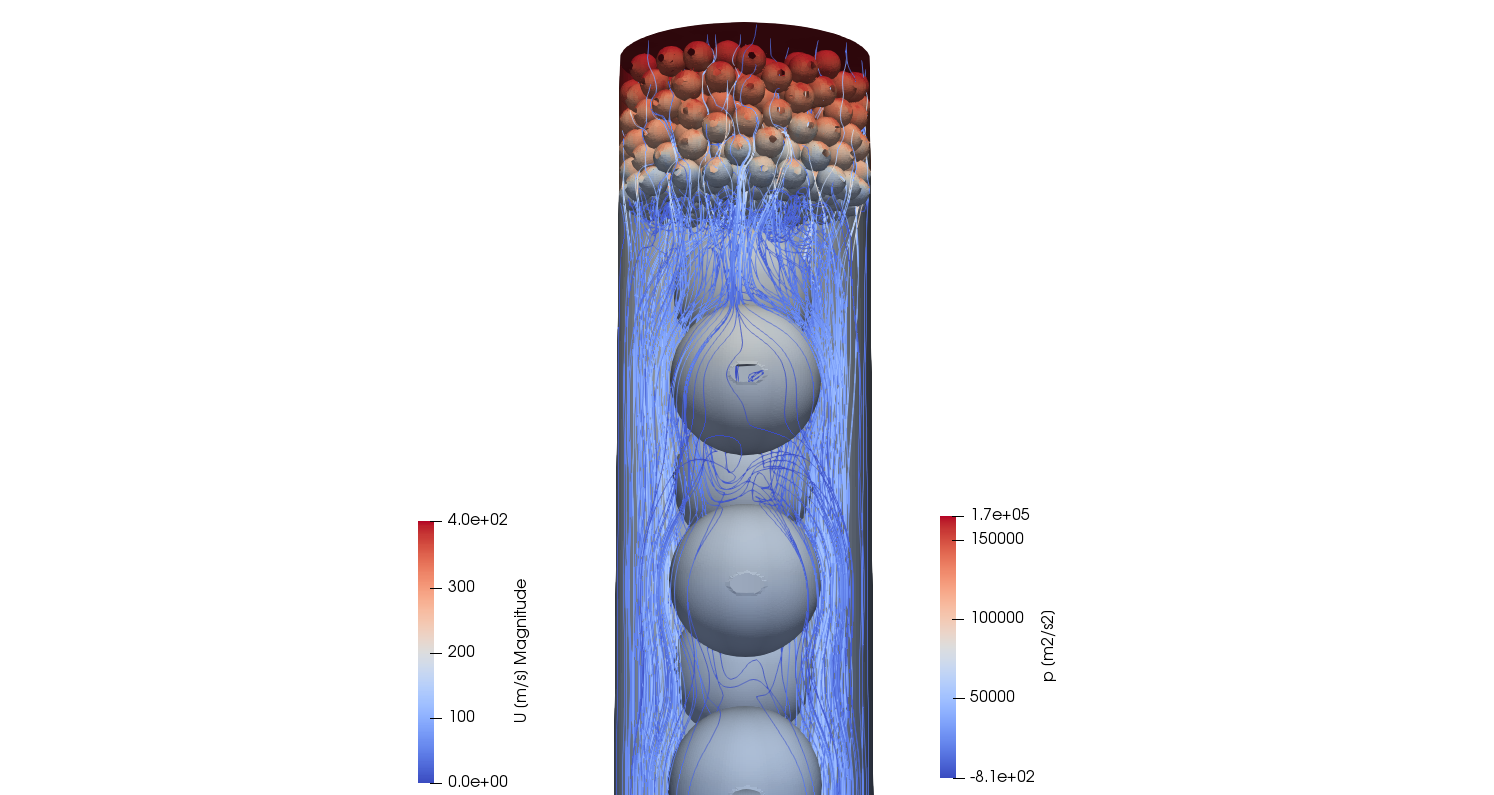
\includegraphics[width=\linewidth]{Figures/visualisation/caseD3/StreamTracer_Sphere_SideView_withunits_CaseD3.png}
	\caption{Side view of case D3 highlighting fluid passing the particles in a straight manner perpendicular
to the plane through the pellet centres.}
	\label{fig:streamtracetube_p_sideview_D3}
\end{figure}
One notable difference between the simulative pressure drop obtained at laminar and turbulent flow would be that the simulative pressure drop approaches values closer to 0 in laminar flow as compared to larger values observed in this work (cf. Fig. \ref{fig:SPSRDiameterAspect}). The greater values of pressure drop associated in this work is owing to a high superficial fluid velocity flowing through the SPSR to achieve turbulent flow. Since pressure drop is directly proportional to superficial velocity (cf. Eq. \ref{eqn:ErgunFromJohanna}), it would stand to reason that greater-than-zero values of pressure drop would be obtained even at high diameter aspect ratios from this work. It should be noted that porosity and diameter aspect ratio are not linearly related with a porosity maximum at D/d = 1.67 \cite{Govindarao1992}.

Lastly, Fig. \ref{fig:SPSRScalingFactor} suggests an increase in pressure drop with increasing scaling factor $s = d/d_A$, opposite of the trend observed previously in laminar flow \cite{Fernengel2020}. The Case E2 present in Fernengel et al.'s study \cite{Fernengel2020} was omitted due to a high time step continuity error, which eventually causes the simulation to crash.
\section{Comparison to Literature}
\subsection{Friction Factor}
\begin{figure} [H]
%\begin{tikzpicture}
%	\begin{axis}[
%								xmode=log,
%								ymode=log,
%								xmin=1500,
%								xmax=35000,
%								ymin=0.1,
%								ymax=500,
%								width=8cm,
%								xtick pos=left,
%								xlabel={wall mod. Reynolds$\ \ \frac{\rho\,u_0\,d_\text{m}}{\eta (1-\varepsilon)}\ / - \ \longrightarrow$},
%								ylabel={friction factor$\ \ \frac{\Delta p}{L} \frac{d_\text{m}}{{\rho\,u_0}^2} \frac{\varepsilon^3}{1-\varepsilon}\ / - \ \longrightarrow$},
%								clip=false,
%								legend cell align=left,
%								legend style={draw=none, font=\small, column sep=0.3em, fill=none, anchor=north west, at={(rel axis cs: 1.05,0.995)}}
%							]
%	\addplot[domain=2431.588115:36473.82173, samples=100, color=TUMBlauDunkel80] {(0.351/(((x/(1-0.56))^0.05)-1.2))*((1-0.56)/0.56^3)};
%	\addlegendentry{Wentz and Thodos}
%	\addplot[domain=2431.588115:36473.82173, samples=100, color=TUMMagenta] {(150+1.75*(x/(1-0.5600619622)))*((1-0.5600619622)^2/(0.5600619622^3*x))};
%	\addlegendentry{Ergun}
%	\addplot[domain=2431.588115:36473.82173, samples=100, color=TUMSchwarz] {6.8*((1-0.5600619622)^1.2/(x^0.2*0.5600619622^3))};
%	\addlegendentry{Hicks}
%	\addplot[domain=2431.588115:36473.82173, samples=100, color=TUMGelbDunkel] {((150+4.2*(x/(1-0.5600619622))^(5/6))*((1-0.5600619622)^2/(0.5600619622^3*x)))};
%	\addlegendentry{Tallmadge}
%	\addplot[domain=2431.588115:36473.82173, samples=100, color=TUMGelbHell] {(276.23+5.05*(x/(1-0.56))^0.87)*((1-0.56)^2/(0.56^3*x))};
%	\addlegendentry{Kuo and Nydegger}
%	\addplot[domain=2431.588115:36473.82173, samples=100, color=TUMBlauAkzent1] {(160+3*(x/(1-0.56))^0.9)*((1-0.56)^2/(0.56^3*x))};
%	\addlegendentry{KTA}
%	\addplot[domain=2431.588115:36473.82173, samples=100, color=TUMElfenbein] {(150+3.89*(x/(1-0.56))^0.87)*((1-0.56)^2/(0.56^3*x))};
%	\addlegendentry{Jones and Krier}
%	\addplot[domain=2431.588115:36473.82173, samples=100, color=TUMGruen] {6.25*((29.32/x)+(1.56/(x^0.4942652816))+0.1)*((1-0.5600619622)^2/(0.5600619622^3))};
%	\addlegendentry{Lee and Ogawa}
%	\addplot[domain=2431.588115:36473.82173, samples=100, color=TUMLila] {(141+1.52*(x/(1-0.56))*(((1-0.56)^2)/(0.56^3*x)))};
%	\addlegendentry{Avontuur and Geldart}
%	\addplot[domain=2431.588115:36473.82173, samples=100, color=TUMBlauDunkel80] {(-13930.7336+4.48*((x/(1-0.5600619622))))*((1-0.5600619622)^2/((0.5600619622^3*x)))};
%	\addlegendentry{O'Neill and Benyahia}
%	\addplot[domain=2431.588115:36473.82173, samples=100, color=TUMBlauDunkel50] {((154*2.212121212+(1/2.579236)*(x/(1-0.5600619622))))*2.212121212*((1-0.5600619622)^2/(0.5600619622^3*x))};
%	\addlegendentry{Eisfeld and Schnitzlein}
%				%\addplot[draw=TUMRotHell, thick] table[x index = 0, restrict x to domain=2431.588115:36473.82173, y index = 1, restrict y to domain=0.5:150, log basis y=10]{Figures/data/TurbulentSimulativeSettings.txt};
%				%\addlegendentry{TurbulentSimulation}
%				\addplot[draw=TUMRotHell, thick] table[x index = 0,y index = 1, log basis y=10]{Figures/data/TurbulentSimulativeSettings.txt};
%				\addlegendentry{TurbulentSimulation}
%	
%\end{axis}
%\end{tikzpicture}

\begin{tikzpicture}
\begin{axis}[
xmode=log,
ymode=log,
xmin=1500,
xmax=40000,
ymin=0.1,
ymax=500,
width=8cm,
xtick pos=left,
xlabel={Normal Reynolds$\ \ \frac{\rho\,u_0\,D}{\mu}\ / - \ \longrightarrow$},
ylabel={friction factor$\ \ \frac{\Delta P}{L} \frac{d_\text{m}}{{\rho\,u_0}^2} \frac{\varepsilon^3}{1-\varepsilon}\ / - \ \longrightarrow$},
clip=false,
legend cell align=left,
legend style={draw=none, font=\small, column sep=0.3em, fill=none, anchor=north west, at={(rel axis cs: 1.05,0.995)}}
]
\addplot[domain=2431.588115:36473.82173, samples=100, color=TUMBlauHell] {(150+1.75*(x/(1-0.5600619622)))*((1-0.5600619622)^2/(0.5600619622^3*x))};
\addlegendentry{Original Ergun Equation}

%Addition of Fp,Ergun for weighting factor counterparts,fw1 and fw2, scatter plot style.
\addplot[only marks, mark = star, mark options={draw=TUMBlau, fill=TUMBlauDunkel, scale=1.4}] table[x index = 0,y index = 1]{Figures/data/fp_weightingfactor_scatterpoints/fp_weightingfactor_wallmodRe_Ergun-fw-1.txt}; \addlegendentry{Ergun with weighting factor, $f_{w,1}$}

\addplot[only marks, mark = otimes*, mark options={draw=TUMBlauHell20, fill=TUMBlauDunkel, scale=0.7}] table[x index = 0,y index = 1]{Figures/data/fp_weightingfactor_scatterpoints/fp_weightingfactor_wallmodRe_Ergun-fw-2.txt}; \addlegendentry{Ergun with weighting factor, $f_{w,2}$}
%End addtion of weighting factor counterparts.

%\addplot[domain=2431.588115:36473.82173, samples=100, color=TUMBlauDunkel80] {(0.351/(((x/(1-0.56))^0.05)-1.2))*((1-0.56)/0.56^3)};
%\addlegendentry{Wentz and Thodos}

%\addplot[domain=2431.588115:36473.82173, samples=100, color=TUMSchwarz] {6.8*((1-0.5600619622)^1.2/(x^0.2*0.5600619622^3))
%};
%\addlegendentry{Hicks}

%\addplot[domain=2431.588115:36473.82173, samples=100, color=TUMGelbDunkel] {((150+4.2*(x/(1-0.5600619622))^(5/6))*((1-0.5600619622)^2/(0.5600619622^3*x)))}; \addlegendentry{Tallmadge}

\addplot[dashed, domain=2431.588115:36473.82173, samples=100, color=TUMGruenDunkel] {(276.23+5.05*(x/(1-0.56))^0.87)*((1-0.56)^2/(0.56^3*x))
}; \addlegendentry{Kuo and Nydegger}

%\addplot[domain=2431.588115:36473.82173, samples=100, color=TUMBlauAkzent1] {(160+3*(x/(1-0.56))^0.9)*((1-0.56)^2/(0.56^3*x))}; \addlegendentry{KTA}

\addplot[domain=2431.588115:36473.82173, samples=100, color=TUMOrange] {(150+3.89*(x/(1-0.56))^0.87)*((1-0.56)^2/(0.56^3*x))
}; \addlegendentry{Jones and Krier}

\addplot[domain=2431.588115:36473.82173, samples=100, color=TUMCyan] {6.25*((29.32/x)+(1.56/(x^0.4942652816))+0.1)*((1-0.5600619622)^2/(0.5600619622^3))}; \addlegendentry{Lee and Ogawa}

\addplot[dash dot, domain=2431.588115:36473.82173, samples=100, color=TUMBlauAkzent2] {(141+1.52*(x)/(1-0.5600619622))*((1-0.5600619622)^2/(0.5600619622^3*x))}; \addlegendentry{Avontuur and Geldart}

\addplot[domain=2431.588115:36473.82173, samples=100, color=TUMMagenta] {(-13930.7336+4.48*(x/(1-0.5600619622)))*((1-0.5600619622)^2/(0.5600619622^3*x))};
\addlegendentry{O'Neill and Benyahia}

%\addplot[domain=2431.588115:36473.82173, samples=100, color=TUMBlauDunkel50] {(154*2.212121212+(1/2.579236)*(x/(1-0.5600619622)))*2.212121212*((1-0.5600619622)^2/(0.5600619622^3*x))};
%\addlegendentry{Eisfeld and Schnitzlein}

%\addplot[domain=2431.588115:36473.82173, samples=100, color=TUMBlauDunkel50] {(180+2.871*((x/(1-0.5600619622)))^0.9)*((1-0.5600619622)^2/(0.5600619622^3*x))};
%\addlegendentry{Carman}

%\addplot[domain=2431.588115:36473.82173, samples=100, color=TUMBlauDunkel50] {(160+3.1*((x/(1-0.5600619622)))^0.9)*((1-0.5600619622)^2/(0.5600619622^3*x))};
%\addlegendentry{Brauer}

%\addplot[domain=2431.588115:36473.82173, samples=100, color=TUMBlauDunkel50] {(368+1.24*((x/(1-0.5600619622))))*((1-0.5600619622)^2/((0.5600619622^3*x)))};
%\addlegendentry{Handley and Heggs}

%\addplot[domain=2431.588115:36473.82173, samples=100, color=TUMBlauDunkel50] {(180+1.8*(x/(1-0.5600619622)))*((1-0.5600619622)^2/(0.5600619622^3*x))};
%\addlegendentry{Macdonald, El-Sayed, Mow and Dullien}


%Scatter Plot of simulative values are below
\addplot[only marks, mark options={color=TUMRotHell, mark=triangle*, scale=0.8}] table[x index = 0,y index = 1, log basis y=10]{Figures/data/NormalReynolds_fp.txt};
\addlegendentry{Simulation}
%end scatter plot of simulative values




%try densely dashed.. approx 5 correlation for readability.
\end{axis}
\end{tikzpicture}
\caption{Simulative and Literature Friction Factor against normal Reynolds number.}%
\label{fig:ComparisonBetweenSimulativeAndLiteratureNormalReFrictionFactor}%

%\begin{tikzpicture}
%	\begin{axis}[
%								xmode=log,
%								ymode=log,
%								xmin=1500,
%								xmax=35000,
%								ymin=0.1,
%								ymax=500,
%								width=8cm,
%								xtick pos=left,
%								xlabel={wall mod. Reynolds$\ \ \frac{\rho\,u_0\,d_\text{m}}{\eta (1-\varepsilon)}\ / - \ \longrightarrow$},
%								ylabel={friction factor$\ \ \frac{\Delta p}{L} \frac{d_\text{m}}{{\rho\,u_0}^2} \frac{\varepsilon^3}{1-\varepsilon}\ / - \ \longrightarrow$},
%								clip=false,
%								legend cell align=left,
%								legend style={draw=none, font=\small, column sep=0.3em, fill=none, anchor=north west, at={(rel axis cs: 1.05,0.995)}}
%							]
%	\addplot[domain=2000:30000, samples=100, color=TUMBlauDunkel80] {(0.351/(((x/(1-0.56))^0.05)-1.2))*((1-0.56)/0.56^3)};
%	\addlegendentry{Wentz and Thodos}
%	\addplot[domain=2000:30000, samples=100, color=TUMMagenta] {(150+1.75*(x/(1-0.5600619622)))*((1-0.5600619622)^2/(0.5600619622^3*x))};
%	\addlegendentry{Ergun}
%	\addplot[domain=2000:30000, samples=100, color=TUMSchwarz] {6.8*((1-0.5600619622)^1.2/(x^0.2*0.5600619622^3))};
%	\addlegendentry{Hicks}
%	\addplot[domain=2000:30000, samples=100, color=TUMGelbDunkel] {((150+4.2*(x/(1-0.5600619622))^(5/6))*((1-0.5600619622)^2/(0.5600619622^3*x)))};
%	\addlegendentry{Tallmadge}
%	\addplot[domain=2000:30000, samples=100, color=TUMGelbHell] {(276.23+5.05*(x/(1-0.56))^0.87)*((1-0.56)^2/(0.56^3*x))};
%	\addlegendentry{Kuo and Nydegger}
%	\addplot[domain=2000:30000, samples=100, color=TUMBlauAkzent1] {(160+3*(x/(1-0.56))^0.9)*((1-0.56)^2/(0.56^3*x))};
%	\addlegendentry{KTA}
%	\addplot[domain=2000:30000, samples=100, color=TUMElfenbein] {(150+3.89*(x/(1-0.56))^0.87)*((1-0.56)^2/(0.56^3*x))};
%	\addlegendentry{Jones and Krier}
%	\addplot[domain=2000:30000, samples=100, color=TUMGruen] {6.25*((29.32/x)+(1.56/(x^0.4942652816))+0.1)*((1-0.5600619622)^2/(0.5600619622^3))};
%	\addlegendentry{Lee and Ogawa}
%	\addplot[domain=2000:30000, samples=100, color=TUMLila] {(141+1.52*(x/(1-0.56))*(((1-0.56)^2)/(0.56^3*x)))};
%	\addlegendentry{Avontuur and Geldart}
%	\addplot[domain=2000:30000, samples=100, color=TUMBlauDunkel80] {(-13930.7336+4.48*((x/(1-0.5600619622))))*((1-0.5600619622)^2/((0.5600619622^3*x)))};
%	\addlegendentry{O'Neill and Benyahia}
%	\addplot[domain=2000:30000, samples=100, color=TUMBlauDunkel50] {((154*2.212121212+(1/2.579236)*(x/(1-0.5600619622))))*2.212121212*((1-0.5600619622)^2/(0.5600619622^3*x))};
%	\addlegendentry{Eisfeld and Schnitzlein}
%				%\addplot[draw=TUMRotHell, thick] table[x index = 0, restrict x to domain=2000:30000, y index = 1, restrict y to domain=0.5:150, log basis y=10]{Figures/data/TurbulentSimulativeSettings.txt};
%				%\addlegendentry{TurbulentSimulation}
%				\addplot[draw=TUMRotHell, thick] table[x index = 0,y index = 1, log basis y=10]{Figures/data/TurbulentSimulativeSettings.txt};
%				\addlegendentry{TurbulentSimulation}
%	
%\end{axis}
%\end{tikzpicture}

\begin{tikzpicture}
\begin{axis}[
xmode=log,
ymode=log,
xmin=1500,
xmax=40000,
ymin=0.1,
ymax=500,
width=8cm,
xtick pos=left,
xlabel={wall mod. Reynolds$\ \ \frac{\rho\,u_0\,d_m}{\eta(1-\epsilon)}\ / - \ \longrightarrow$},
ylabel={friction factor$\ \ \frac{\Delta P}{L} \frac{d_\text{m}}{{\rho\,u_0}^2} \frac{\varepsilon^3}{1-\varepsilon}\ / - \ \longrightarrow$},
clip=false,
legend cell align=left,
legend style={draw=none, font=\small, column sep=0.3em, fill=none, anchor=north west, at={(rel axis cs: 1.05,0.995)}}
]
%\addplot[domain=2000:30000, samples=100, color=TUMMagenta] {(150+1.75*(x/(1-0.5600619622)))*((1-0.5600619622)^2/(0.5600619622^3*x))};
%\addlegendentry{Original Ergun Equation}
%think about how to place this in turbulent flow ltr

%\addplot[domain=2000:30000, samples=100, color=TUMMagenta] {(150+1.75*(x/(1-0.5600619622)))*((1-0.5600619622)^2/(0.5600619622^3*x))};
%\addlegendentry{Ergun with fw1}
%think about how to place this in turbulent flow ltr

%\addplot[domain=2000:30000, samples=100, color=TUMMagenta] {(150+1.75*(x/(1-0.5600619622)))*((1-0.5600619622)^2/(0.5600619622^3*x))};
%\addlegendentry{Ergun with fw2}
%think about how to place this in turbulent flow ltr

%\addplot[domain=2000:30000, samples=100, color=TUMBlauDunkel80] {(0.351/(((x/(1-0.56))^0.05)-1.2))*((1-0.56)/0.56^3)};
%\addlegendentry{Wentz and Thodos}

%\addplot[domain=2000:30000, samples=100, color=TUMSchwarz] {6.8*((1-0.5600619622)^1.2/(x^0.2*0.5600619622^3))
%};
%\addlegendentry{Hicks}

%\addplot[domain=2000:30000, samples=100, color=TUMGelbDunkel] {((150+4.2*(x/(1-0.5600619622))^(5/6))*((1-0.5600619622)^2/(0.5600619622^3*x)))}; \addlegendentry{Tallmadge}

\addplot[domain=2431.588115:36473.82173, samples=100, color=TUMBlauHell] {(150+1.75*(x/(1-0.5600619622)))*((1-0.5600619622)^2/(0.5600619622^3*x))};
\addlegendentry{Original Ergun Equation}

%Addition of Fp,Ergun for weighting factor counterparts,fw1 and fw2, scatter plot style.
\addplot[only marks, mark = star, mark options={draw=TUMBlau, fill=TUMBlauDunkel, scale=1.4}] table[x index = 0,y index = 1]{Figures/data/fp_weightingfactor_scatterpoints/fp_weightingfactor_wallmodRe_Ergun-fw-1.txt}; \addlegendentry{Ergun with weighting factor, $f_{w,1}$}

\addplot[only marks, mark = otimes*, mark options={draw=TUMBlauHell20, fill=TUMBlauDunkel, scale=0.7}] table[x index = 0,y index = 1]{Figures/data/fp_weightingfactor_scatterpoints/fp_weightingfactor_wallmodRe_Ergun-fw-2.txt}; \addlegendentry{Ergun with weighting factor, $f_{w,2}$}
%End addtion of weighting factor counterparts.



\addplot[dashed, color=TUMGruenDunkel, domain=2000:30000, samples=100] {(276.23+5.05*(x/(1-0.56))^0.87)*((1-0.56)^2/(0.56^3*x))
}; \addlegendentry{Kuo and Nydegger}

%\addplot[domain=2000:30000, samples=100, color=TUMBlauAkzent1] {(160+3*(x/(1-0.56))^0.9)*((1-0.56)^2/(0.56^3*x))}; \addlegendentry{KTA}

\addplot[domain=2000:30000, samples=100, color=TUMOrange] {(150+3.89*(x/(1-0.56))^0.87)*((1-0.56)^2/(0.56^3*x))
}; \addlegendentry{Jones and Krier}

\addplot[domain=2000:30000, samples=100, color=TUMCyan] {6.25*((29.32/x)+(1.56/(x^0.4942652816))+0.1)*((1-0.5600619622)^2/(0.5600619622^3))}; \addlegendentry{Lee and Ogawa}

\addplot[dash dot, color=TUMBlauAkzent2, domain=2000:30000, samples=100] {(141+1.52*(x)/(1-0.5600619622))*((1-0.5600619622)^2/(0.5600619622^3*x))}; \addlegendentry{Avontuur and Geldart}

\addplot[domain=2000:30000, samples=100, color=TUMMagenta] {(-13930.7336+4.48*(x/(1-0.5600619622)))*((1-0.5600619622)^2/(0.5600619622^3*x))};
\addlegendentry{O'Neill and Benyahia}

%\addplot[domain=2000:30000, samples=100, color=TUMBlauDunkel50] {(154*2.212121212+(1/2.579236)*(x/(1-0.5600619622)))*2.212121212*((1-0.5600619622)^2/(0.5600619622^3*x))};
%\addlegendentry{Eisfeld and Schnitzlein}

%\addplot[domain=2000:30000, samples=100, color=TUMBlauDunkel50] {(180+2.871*((x/(1-0.5600619622)))^0.9)*((1-0.5600619622)^2/(0.5600619622^3*x))};
%\addlegendentry{Carman}

%\addplot[domain=2000:30000, samples=100, color=TUMBlauDunkel50] {(160+3.1*((x/(1-0.5600619622)))^0.9)*((1-0.5600619622)^2/(0.5600619622^3*x))};
%\addlegendentry{Brauer}

%\addplot[domain=2000:30000, samples=100, color=TUMBlauDunkel50] {(368+1.24*((x/(1-0.5600619622))))*((1-0.5600619622)^2/((0.5600619622^3*x)))};
%\addlegendentry{Handley and Heggs}

%\addplot[domain=2000:30000, samples=100, color=TUMBlauDunkel50] {(180+1.8*(x/(1-0.5600619622)))*((1-0.5600619622)^2/(0.5600619622^3*x))};
%\addlegendentry{Macdonald, El-Sayed, Mow and Dullien}

%Scatter Plot of simulative values are below
\addplot[only marks, mark options={color=TUMRotHell, mark=triangle*, scale=0.8}] table[x index = 0,y index = 1, log basis y=10]{Figures/data/WallModReynolds_fp.txt};
\addlegendentry{Simulation}
%end scatter plot of simulative values

%try densely dashed.. approx 5 correlation for readability.
\end{axis}
\end{tikzpicture}
\caption{Simulative and Literature Friction Factor against wall modified Reynolds number.}%
\label{fig:ComparisonBetweenSimulativeAndLiteratureWallModReFrictionFactor}%
%wallmodRe still requires addition of ergun with fw1 and fw2
\end{figure}
With reference to both Figs. \ref{fig:ComparisonBetweenSimulativeAndLiteratureNormalReFrictionFactor} and \ref{fig:ComparisonBetweenSimulativeAndLiteratureWallModReFrictionFactor}, it can be seen that the friction factor correlation as provided by Avontuur and Geldart, Kuo and Nydegger and Ergun are the most similar to the simulative friction factors obtained, with Kuo and Nydegger deviating from the simulative friction factor after a wall modified Reynolds value of \num{5e3}. As mentioned by Jones and Krier, the experiments carried out by Kuo and Nydegger were performed inside a very small diameter tube having a small container diameter to bead diameter ratio ($D/d$) in which frictional wall effects are present \cite{Jones1983}. This also meant that experiments carried out by Kuo and Nydegger were somewhat carried out in a SPSR-like environment similar to this study as the "data obtained for a test chamber diameter was too small for the bead diameter" \cite{Jones1983}. Hence, this would attest to its similarity with the simulative friction factor.

The deviation from simulative friction factor observed beyond a wall modified Reynolds value of \num{5e3} for Kuo and Nydegger would be due to the fact it is approaching (and eventually will) surpass its range of validity for friction factor ($460 < Re <14600$), hence it starts to behave abnormally as it approaches its upper friction factor limit.

Despite being outside its range of applicability, the friction factor provided by the Ergun equation (ref. Tab. \ref{tab:PressureDropFlowRelationsPowderTech}, Figs. \ref{fig:ComparisonBetweenSimulativeAndLiteratureNormalReFrictionFactor} and \ref{fig:ComparisonBetweenSimulativeAndLiteratureWallModReFrictionFactor}) lands close to the simulative friction factor obtained, with a slight over-prediction in friction factor values. A possible explanation for this would be the similarity between the friction factor equation applied in this study (cf. Eq. \ref{eqn:SimulativeFrictionFactor}) and the Ergun equation. The friction factor utilised in this work, as well as those enforced by Avontuur and Geldart, Kuo and Nydegger, Jones and Krier are Ergun-based correlations. Accordingly, each of them are based off the Ergun equation with changes made mostly to the Ergun coefficients and to the related exponents. Looking at both Figs. \ref{fig:ComparisonBetweenSimulativeAndLiteratureNormalReFrictionFactor} and \ref{fig:ComparisonBetweenSimulativeAndLiteratureWallModReFrictionFactor}, friction factors obtained from these Ergun-based correlations are the most similar to simulative results.
Thus, it is plausible that the Ergun equation is largely similar to simulative friction factor values for the reason that the simulative friction factor is a Ergun-based correlation.

On the opposite end of the spectrum, a comparison with the friction factor correlation provided by Lee and Ogawa against the simulative values points to it severely under-predicting the friction factor obtained from simulations. In an attempt to create a correlation that holds true over a wide range of Reynolds number and has a simple physical meaning, Lee and Ogawa \cite{Lee1994} proposed an all-encompassing coefficient for a packed bed to include the effects of Reynolds number and various parameters, with the assumption that flow behaviour is represented by $Re^{-n}$, with $n$ being a function of voidage ($\epsilon$). Though the proposed correlation was largely valid in laminar flow ($1 < Re < 1000$), greater mean errors of upwards to 40\% were observed in turbulent flow ($10^3 < Re < 10^6$) with respect to experimental data \cite{Lee1994}. Thus, its deviation from simulative friction factor values became apparent.

A reason for the extreme deviation from simulative friction factor observed in O'Neill and Benyahia was due to the fact that the $D/d$ value used in the base case A was outside the valid range of 5 < D/dp < 25 suitable for use in O'Neill and Benyahia. This correlation was initially included for the sole purpose of demonstrating what would happen should a correlation be applied outside its range of applicability for its friction factor. However, interestingly enough, its corresponding pressure drop correlation values is the closest to parity when viewed on a parity plot in Fig. \ref{fig:ParityPlotWallModReInTurbulentRegion} in the next subsection.

Furthermore, it is important to note that the friction factor correlations provided by Erdim et al. \cite{Erdim2015} are mostly valid for normal Reynolds, and not wall modified Reynolds. As such, the data presented in Fig. \ref{fig:ComparisonBetweenSimulativeAndLiteratureWallModReFrictionFactor} may not be an entirely fair comparison of between simulative and literature friction factor values. However, a plot of friction factor against normal Reynolds has also shown similar trends (Fig. \ref{fig:ComparisonBetweenSimulativeAndLiteratureNormalReFrictionFactor}), indicating that plotting the friction factor against wall modified Reynolds or normal Reynolds will not drastically affect observed trends.

Viewing both Fig. \ref{fig:ComparisonBetweenSimulativeAndLiteratureWallModReFrictionFactor} and \ref{fig:ComparisonBetweenSimulativeAndLiteratureNormalReFrictionFactor}, it was found that the original Ergun equation and its weighting factor counterparts overestimate the friction factor relative to the simulative values obtained in turbulent flow. Also, the effects of applying a weighting factor on the Ergun equation (be it $f_{w,1}$ or $f_{w,2}$) for the calculation of friction factor appears to be minimal, yielding similar, if not equal to results obtained with the original Ergun equation. However, the consequence of applying weighting factors on the Ergun equation is much more impactful when computing for pressure drop and will be elaborated further below.

It is unfortunate however, that the article for O'Neill and Benyahia, Avontuur and Geldart, Kuo and Nydegger, Ergun could not be retrieved. As such, it is difficult to explain their deviation (or similarities) to the simulative friction factor obtained.
\subsection{Parity Plots}
\begin{figure} [H]
\begin{tikzpicture}
	\begin{axis}[
								xmode=log,
								ymode=log,
								xmin=4E7,
								xmax=1.2E10,
								ymin=1E6,
								ymax=2E10,
								width=10cm,
								xtick pos=left,
								xlabel={pressure drop by simulation$\ \ \big[\frac{\Delta P}{L}\big]_{sim}\  /\ \si{\pascal\per\metre} \ \longrightarrow$},
								ylabel={pressure drop by correlation$\ \ \big[\frac{\Delta P}{L}\big]_{cor}\  /\ \si{\pascal\per\metre} \ \longrightarrow$},
								clip=false,
								legend cell align=left,
								legend style={draw=none, font=\small, column sep=0.3em, fill=none, anchor=north west, at={(rel axis cs: 1.05,0.995)}}
							]
\addplot[only marks, mark = circle*, mark options={color=TUMBlauHell, mark=otimes*, scale=1.2}] table[x index = 0,y index = 1]{Figures/parityplotnormalre/ErgunPdropCor_Nre.txt}; \addlegendentry{Original Ergun Equation}
			
%						\addplot[only marks, mark = diamond*, mark options={draw=TUMBlauDunkel, fill=TUMBlauDunkel, scale=1.4}] table[x index = 0,y index = 1]{Figures/parityplotnormalre/WentzThodosPdropCor_Nre.txt}; \addlegendentry{WentzThodos}
						
%						\addplot[only marks, mark = diamond*, mark options={draw=TUMBlauDunkel, fill=TUMBlauDunkel, scale=1.4}] table[x index = 0,y index = 1]{Figures/parityplotnormalre/HicksPdropCor_Nre.txt}; \addlegendentry{Hicks}
						
%						\addplot[only marks, mark = diamond*, mark options={draw=TUMBlauDunkel, fill=TUMBlauDunkel, scale=1.4}] table[x index = 0,y index = 1]{Figures/parityplotnormalre/TallmadgePdropCor_Nre.txt}; \addlegendentry{Tallmadge}
						
\addplot[only marks, mark = star, mark options={draw=TUMBlau, fill=TUMBlauDunkel, scale=1.4}] table[x index = 0,y index = 1]{Figures/parityplotnormalre/KuoNydeggerPdropCor_Nre.txt}; \addlegendentry{Kuo and Nydegger}
						
%						\addplot[only marks, mark = diamond*, mark options={draw=TUMBlauDunkel, fill=TUMBlauDunkel, scale=1.4}] table[x index = 0,y index = 1]{Figures/parityplotnormalre/KTAPdropCor_Nre.txt}; \addlegendentry{KTA}
						
\addplot[only marks, mark = diamond*, mark options={draw=TUMElfenbein, fill=TUMBlauDunkel, scale=1.4}] table[x index = 0,y index = 1]{Figures/parityplotnormalre/JonesKrierPdropCor_Nre.txt}; \addlegendentry{Jones and Krier}
						
\addplot [only marks, color=TUMMagenta, mark=star] table[x index = 0,y index = 1]{Figures/parityplotnormalre/LeeOgawaPdropCor_Nre.txt}; \addlegendentry{Lee and Ogawa}
						
\addplot[only marks, mark = triangle*, mark options={color=TUMBlauHell, scale=1}] table[x index = 0,y index = 1]{Figures/parityplotnormalre/AvontuurGeldartPdropCor_Nre.txt}; \addlegendentry{Avontuur and Geldart}
						
\addplot[only marks, mark = diamond*, mark options={draw=TUMGruenDunkel, fill=TUMGruenDunkel, scale=1.4}] table[x index = 0,y index = 1]{Figures/parityplotnormalre/OneillBenyahiaPdropCor_Nre.txt}; \addlegendentry{O'Neill and Benyahia}
						
%						\addplot[only marks, mark = diamond*, mark options={draw=TUMBlauDunkel, fill=TUMBlauDunkel, scale=1.4}] table[x index = 0,y index = 1]{Figures/parityplotnormalre/EisfeldSchnitzleinPdropCor_Nre.txt}; \addlegendentry{EisfeldSchnitzlein}
						
						% draw the diagonal
        	\addplot[domain=4E7:1.2E10, samples=2, color=TUMSchwarz] {x}; \addlegendentry{Parity}
        	%draw the 10% envelope for upper and lower limit
        	\addplot[dashed, domain=4E7:1.2E10, samples=2, color=TUMSchwarz] {0.9*x};
        	\addplot[dashed, domain=4E7:1.2E10, samples=2, color=TUMSchwarz] {1.1*x};
        	\addlegendentry{10\% envelope}
        	%draw the 50% envelope upper and lower limit
        	\addplot[dotted, domain=4E7:1.2E10, samples=2, color=TUMSchwarz] {0.5*x};
        	\addplot[dotted, domain=4E7:1.2E10, samples=2, color=TUMSchwarz] {1.5*x};
        	\addlegendentry{50\% envelope}
\end{axis}
\end{tikzpicture}%
	\caption[Parity plot for normal Reynolds in turbulent region, correlations as displayed by Erdim et al.]{Parity plot for normal Reynolds in turbulent region, correlations obtained from Erdim et al. \cite{Erdim2015}.}%
	\label{fig:ParityPlotNormalReInTurbulentRegion}%
		
\begin{tikzpicture}
\begin{axis}[
xmode=log,
ymode=log,
xmin=4E7,
xmax=2E10,
ymin=1.5E6,
ymax=3E10,
width=10cm,
xtick pos=left,
xlabel={pressure drop by simulation$\ \ \big[\frac{\Delta P}{L}\big]_{sim}\  /\ \si{\pascal\per\metre} \ \longrightarrow$},
								ylabel={pressure drop by correlation$\ \ \big[\frac{\Delta P}{L}\big]_{cor}\  /\ \si{\pascal\per\metre} \ \longrightarrow$},
clip=false,
legend cell align=left,
legend style={draw=none, font=\small, column sep=0.3em, fill=none, anchor=north west, at={(rel axis cs: 1.05,0.995)}}
]
\addplot[only marks, mark options={color=TUMElfenbein, mark=otimes*, scale=1.7}] table[x index = 0,y index = 1]{Figures/parityplotwallmodre/ErgunWithModifiedDiameterPdropCor_wallmodre.txt}; \addlegendentry{Ergun with modified diameter, $f_{w,1}$}

\addplot[only marks, mark = otimes*, mark options={draw=TUMBlauHell20, fill=TUMBlauDunkel, scale=1.0}] table[x index = 0,y index = 1]{Figures/parityplotwallmodre/Ergun_fw2_PdropCor_wallmodre.txt}; \addlegendentry{Ergun with weighting factor, $f_{w,2}$}

\addplot[only marks, mark = circle*, mark options={color=TUMBlauHell, mark=otimes*, scale=1.2}] table[x index = 0,y index = 1]{Figures/parityplotwallmodre/OriginalErgunPdropCor_wallmodre.txt}; \addlegendentry{Original Ergun Equation}

%\addplot[only marks, mark = diamond*, mark options={draw=TUMBlauHell50, fill=TUMBlauDunkel, scale=1.4}] table[x index = 0,y index = 1]{Figures/parityplotwallmodre/WentzThodosPdropCor_wallmodre.txt}; \addlegendentry{WentzThodos}

%\addplot[only marks, mark = diamond*, mark options={draw=TUMBlauHell80, fill=TUMBlauDunkel, scale=1.4}] table[x index = 0,y index = 1]{Figures/parityplotwallmodre/HicksPdropCor_wallmodre.txt}; \addlegendentry{Hicks}

%\addplot[only marks, mark = diamond*, mark options={draw=TUMBlauHell, fill=TUMBlauDunkel, scale=1.4}] table[x index = 0,y index = 1]{Figures/parityplotwallmodre/TallmadgePdropCor_wallmodre.txt}; \addlegendentry{Tallmadge}

\addplot[only marks, mark = star, mark options={draw=TUMBlau, fill=TUMBlauDunkel, scale=1.4}] table[x index = 0,y index = 1]{Figures/parityplotwallmodre/KuoNydeggerPdropCor_wallmodre.txt}; \addlegendentry{Kuo and Nydegger}

%\addplot[only marks, mark = diamond*, mark options={draw=TUMOrange, fill=TUMBlauDunkel, scale=1.4}] table[x index = 0,y index = 1]{Figures/parityplotwallmodre/KTAPdropCor_wallmodre.txt}; \addlegendentry{KTA}

\addplot[only marks, mark = diamond*, mark options={draw=TUMElfenbein, fill=TUMBlauDunkel, scale=1.4}] table[x index = 0,y index = 1]{Figures/parityplotwallmodre/JonesKrierPdropCor_wallmodre.txt}; \addlegendentry{Jones and Krier}

\addplot [only marks, color=TUMMagenta, mark=star] table[x index = 0,y index = 1]{Figures/parityplotwallmodre/LeeOgawaPdropCor_wallmodre.txt}; \addlegendentry{Lee and Ogawa}

\addplot[only marks, mark = triangle*, mark options={color=TUMBlauHell, scale=1}] table[x index = 0,y index = 1]{Figures/parityplotwallmodre/AvontuurGeldartPdropCor_wallmodre.txt}; \addlegendentry{Avontuur and Geldart}

\addplot[only marks, mark = diamond*, mark options={draw=TUMGruenDunkel, fill=TUMGruenDunkel, scale=1.4}] table[x index = 0,y index = 1]{Figures/parityplotwallmodre/OneillBenyahiaPdropCor_wallmodre.txt}; \addlegendentry{O'Neill and Benyahia}

\addplot[only marks, mark = star, mark options={draw=TUMGruen, fill=TUMGruen, scale=1}] table[x index = 0,y index = 1]{Figures/parityplotwallmodre/MacdonaldEl-SayedMowDullienPdropCor_wallmodre.txt}; \addlegendentry{Macdonald et al.}

%\addplot[only marks, mark = diamond*, mark options={draw=TUMRotHell, fill=TUMBlauDunkel, scale=1.4}] table[x index = 0,y index = 1]{Figures/parityplotwallmodre/EisfeldSchnitzleinPdropCor_wallmodre.txt}; \addlegendentry{EisfeldSchnitzlein}

%\addplot[only marks, mark = diamond*, mark options={draw=TUMRotHell, fill=TUMBlauDunkel, scale=1.4}] table[x index = 0,y index = 1]{Figures/parityplotwallmodre/CarmanPdropCor_wallmodre.txt}; \addlegendentry{Carman}

%\addplot[only marks, mark = diamond*, mark options={draw=TUMRotHell, fill=TUMBlauDunkel, scale=1.4}] table[x index = 0,y index = 1]{Figures/parityplotwallmodre/BrauerPdropCor_wallmodre.txt}; \addlegendentry{Brauer}

%\addplot[only marks, mark = diamond*, mark options={draw=TUMRotHell, fill=TUMBlauDunkel, scale=1.4}] table[x index = 0,y index = 1]{Figures/parityplotwallmodre/HandleyandHeggsPdropCor_wallmodre.txt}; \addlegendentry{Handley and Heggs}

%\addplot[only marks, mark = diamond*, mark options={color=TUMBlauHell, scale=1.4}] table[x index = 0,y index = 1]{Figures/parityplotwallmodre/MacdonaldEl-SayedMowDullienPdropCor_wallmodre.txt}; \addlegendentry{Macdonald, El-Sayed, Mow, Dullien}

%Now comparing Cases D1, D2 and D3 pdrop in wall mod. Reynolds
\addplot[only marks, mark = square*, mark options={draw=TUMOrange, fill=TUMOrange, scale=0.5}] table[x index = 0,y index = 1]{Figures/parityplotwallmodre/D1PdropCor_wallmodre.txt}; \addlegendentry{D1 with Ergun correlation}

\addplot[only marks, mark = square*, mark options={draw=TUMGrau50, fill=TUMGrau50, scale=0.5}] table[x index = 0,y index = 1]{Figures/parityplotwallmodre/D2PdropCor_wallmodre.txt}; \addlegendentry{D2 with Ergun correlation}

\addplot[only marks, mark = square*, mark options={draw=TUMGrau20, fill=TUMGrau20, scale=0.5}] table[x index = 0,y index = 1]{Figures/parityplotwallmodre/D3PdropCor_wallmodre.txt}; \addlegendentry{D3 with Ergun correlation}











% draw the diagonal
\addplot[domain=4E7:2E10, samples=2, color=TUMSchwarz] {x}; \addlegendentry{Parity}
%draw the 10% envelope for upper and lower limit
\addplot[dashed, domain=4E7:2E10, samples=2, color=TUMSchwarz] {0.9*x};
\addplot[dashed, domain=4E7:2E10, samples=2, color=TUMSchwarz] {1.1*x};
\addlegendentry{10\% envelope}
%draw the 50% envelope upper and lower limit
\addplot[dotted, domain=4E7:2E10, samples=2, color=TUMSchwarz] {0.5*x};
\addplot[dotted, domain=4E7:2E10, samples=2, color=TUMSchwarz] {1.5*x};
\addlegendentry{50\% envelope}
\end{axis}
\end{tikzpicture}%
	\caption[Parity plot for wall modified Reynolds in turbulent region, correlations as displayed by Erdim et al.]{Parity plot for wall modified Reynolds in turbulent region, correlations obtained from Erdim et al. \cite{Erdim2015}.}%
	\label{fig:ParityPlotWallModReInTurbulentRegion}%
	
\end{figure}

\begin{figure} [H]
\begin{tikzpicture}
\begin{axis}[
xmode=log,
ymode=log,
xmin=4E7,
xmax=2E10,
ymin=1.5E6,
ymax=3E10,
width=10cm,
xtick pos=left,
xlabel={pressure drop by simulation$\ \ \big[\frac{\Delta P}{L}\big]_{sim}\  /\ \si{\pascal\per\metre} \ \longrightarrow$},
								ylabel={pressure drop by correlation$\ \ \big[\frac{\Delta P}{L}\big]_{cor}\  /\ \si{\pascal\per\metre} \ \longrightarrow$},
clip=false,
legend cell align=left,
legend style={draw=none, font=\small, column sep=0.3em, fill=none, anchor=north west, at={(rel axis cs: 1.05,0.995)}}
]
%\addplot[only marks, mark options={color=TUMElfenbein, mark=otimes*, scale=1.7}] table[x index = 0,y index = 1]{Figures/parityplotwallmodre/ErgunWithModifiedDiameterPdropCor_wallmodre.txt}; \addlegendentry{Ergun with modified diameter, $f_{w,1}$}

%\addplot[only marks, mark = otimes*, mark options={draw=TUMBlauHell20, fill=TUMBlauDunkel, scale=1.0}] table[x index = 0,y index = 1]{Figures/parityplotwallmodre/Ergun_fw2_PdropCor_wallmodre.txt}; \addlegendentry{Ergun with weighting factor, $f_{w,2}$}

%\addplot[only marks, mark = circle*, mark options={color=TUMBlauHell, mark=otimes*, scale=1.2}] table[x index = 0,y index = 1]{Figures/parityplotwallmodre/OriginalErgunPdropCor_wallmodre.txt}; \addlegendentry{Original Ergun Equation}

%\addplot[only marks, mark = diamond*, mark options={draw=TUMBlauHell50, fill=TUMBlauDunkel, scale=1.4}] table[x index = 0,y index = 1]{Figures/parityplotwallmodre/WentzThodosPdropCor_wallmodre.txt}; \addlegendentry{WentzThodos}

%\addplot[only marks, mark = diamond*, mark options={draw=TUMBlauHell80, fill=TUMBlauDunkel, scale=1.4}] table[x index = 0,y index = 1]{Figures/parityplotwallmodre/HicksPdropCor_wallmodre.txt}; \addlegendentry{Hicks}

%\addplot[only marks, mark = diamond*, mark options={draw=TUMBlauHell, fill=TUMBlauDunkel, scale=1.4}] table[x index = 0,y index = 1]{Figures/parityplotwallmodre/TallmadgePdropCor_wallmodre.txt}; \addlegendentry{Tallmadge}

%\addplot[only marks, mark = star, mark options={draw=TUMBlau, fill=TUMBlauDunkel, scale=1.4}] table[x index = 0,y index = 1]{Figures/parityplotwallmodre/KuoNydeggerPdropCor_wallmodre.txt}; \addlegendentry{Kuo and Nydegger}

%\addplot[only marks, mark = diamond*, mark options={draw=TUMOrange, fill=TUMBlauDunkel, scale=1.4}] table[x index = 0,y index = 1]{Figures/parityplotwallmodre/KTAPdropCor_wallmodre.txt}; \addlegendentry{KTA}

%\addplot[only marks, mark = diamond*, mark options={draw=TUMElfenbein, fill=TUMBlauDunkel, scale=1.4}] table[x index = 0,y index = 1]{Figures/parityplotwallmodre/JonesKrierPdropCor_wallmodre.txt}; \addlegendentry{Jones and Krier}

%\addplot [only marks, color=TUMMagenta, mark=star] table[x index = 0,y index = 1]{Figures/parityplotwallmodre/LeeOgawaPdropCor_wallmodre.txt}; \addlegendentry{Lee and Ogawa}

%\addplot[only marks, mark = triangle*, mark options={color=TUMBlauHell, scale=1}] table[x index = 0,y index = 1]{Figures/parityplotwallmodre/AvontuurGeldartPdropCor_wallmodre.txt}; \addlegendentry{Avontuur and Geldart}

%\addplot[only marks, mark = diamond*, mark options={draw=TUMGruenDunkel, fill=TUMGruenDunkel, scale=1.4}] table[x index = 0,y index = 1]{Figures/parityplotwallmodre/OneillBenyahiaPdropCor_wallmodre.txt}; \addlegendentry{O'Neill and Benyahia}

%\addplot[only marks, mark = star, mark options={draw=TUMGruen, fill=TUMGruen, scale=1}] table[x index = 0,y index = 1]{Figures/parityplotwallmodre/MacdonaldEl-SayedMowDullienPdropCor_wallmodre.txt}; \addlegendentry{Macdonald et al.}

%\addplot[only marks, mark = diamond*, mark options={draw=TUMRotHell, fill=TUMBlauDunkel, scale=1.4}] table[x index = 0,y index = 1]{Figures/parityplotwallmodre/EisfeldSchnitzleinPdropCor_wallmodre.txt}; \addlegendentry{EisfeldSchnitzlein}

%\addplot[only marks, mark = diamond*, mark options={draw=TUMRotHell, fill=TUMBlauDunkel, scale=1.4}] table[x index = 0,y index = 1]{Figures/parityplotwallmodre/CarmanPdropCor_wallmodre.txt}; \addlegendentry{Carman}

%\addplot[only marks, mark = diamond*, mark options={draw=TUMRotHell, fill=TUMBlauDunkel, scale=1.4}] table[x index = 0,y index = 1]{Figures/parityplotwallmodre/BrauerPdropCor_wallmodre.txt}; \addlegendentry{Brauer}

%\addplot[only marks, mark = diamond*, mark options={draw=TUMRotHell, fill=TUMBlauDunkel, scale=1.4}] table[x index = 0,y index = 1]{Figures/parityplotwallmodre/HandleyandHeggsPdropCor_wallmodre.txt}; \addlegendentry{Handley and Heggs}

%\addplot[only marks, mark = diamond*, mark options={color=TUMBlauHell, scale=1.4}] table[x index = 0,y index = 1]{Figures/parityplotwallmodre/MacdonaldEl-SayedMowDullienPdropCor_wallmodre.txt}; \addlegendentry{Macdonald, El-Sayed, Mow, Dullien}

%Now comparing Cases D1, D2 and D3 w/out weighting factors in wall mod. Reynolds
%\addplot[only marks, mark = square*, mark options={draw=TUMOrange, fill=TUMOrange, scale=0.5}] table[x index = 0,y index = 1]{Figures/parityplotwallmodre/D1PdropCor_wallmodre.txt}; \addlegendentry{D1 with Ergun correlation}
%
%\addplot[only marks, mark = square*, mark options={draw=TUMGrau50, fill=TUMGrau50, scale=0.5}] table[x index = 0,y index = 1]{Figures/parityplotwallmodre/D2PdropCor_wallmodre.txt}; \addlegendentry{D2 with Ergun correlation}
%
%\addplot[only marks, mark = square*, mark options={draw=TUMGrau20, fill=TUMGrau20, scale=0.5}] table[x index = 0,y index = 1]{Figures/parityplotwallmodre/D3PdropCor_wallmodre.txt}; \addlegendentry{D3 with Ergun correlation}
%end comparison

%now comparing Case D1 with weighting factor in wall mod. Reynolds
\addplot[only marks, mark = otimes*, mark options={draw=TUMOrange, fill=TUMOrange, scale=0.7}] table[x index = 0,y index = 1]{Figures/parityplotwallmodre/comparisonwithvaryingdiameteraspectratio/D1/D1PdropCor_wallmodre_ErgunWithfw1.txt}; \addlegendentry{D1 with Ergun correlation, $f_{w,1}$}

\addplot[only marks, mark = otimes*, mark options={draw=TUMGelbHell, fill=TUMGelbHell, scale=0.7}] table[x index = 0,y index = 1]{Figures/parityplotwallmodre/comparisonwithvaryingdiameteraspectratio/D1/D1PdropCor_wallmodre_ErgunWithfw2.txt}; \addlegendentry{D1 with Ergun correlation, $f_{w,2}$}
%end comparison

%now comparing Case D2 with weighting factor in wall mod. Reynolds
\addplot[only marks, mark = triangle*, mark options={draw=TUMBlauAkzent1, fill=TUMBlauAkzent1, scale=1}] table[x index = 0,y index = 1]{Figures/parityplotwallmodre/comparisonwithvaryingdiameteraspectratio/D2/D2PdropCor_wallmodre_ErgunWithfw1.txt}; \addlegendentry{D2 with Ergun correlation, $f_{w,1}$}

\addplot[only marks, mark = star, mark options={draw=TUMBlauAkzent2, fill=TUMBlauAkzent2, scale=1.5}] table[x index = 0,y index = 1]{Figures/parityplotwallmodre/comparisonwithvaryingdiameteraspectratio/D2/D2PdropCor_wallmodre_ErgunWithfw2.txt}; \addlegendentry{D2 with Ergun correlation, $f_{w,2}$}
%end comparison


%now comparing Case D3 with weighting factor in wall mod. Reynolds
\addplot[only marks, mark = star, mark options={draw=TUMBlauDunkel80, fill=TUMBlauDunkel80, scale=1.5}] table[x index = 0,y index = 1]{Figures/parityplotwallmodre/comparisonwithvaryingdiameteraspectratio/D3/D3PdropCor_wallmodre_ErgunWithfw1.txt}; \addlegendentry{D3 with Ergun correlation, $f_{w,1}$}

\addplot[only marks, mark = diamond*, mark options={draw=TUMBlauDunkel50, fill=TUMBlauDunkel50, scale=1}] table[x index = 0,y index = 1]{Figures/parityplotwallmodre/comparisonwithvaryingdiameteraspectratio/D3/D3PdropCor_wallmodre_ErgunWithfw1.txt}; \addlegendentry{D3 with Ergun correlation, $f_{w,2}$}
%end comparison


% draw the diagonal
\addplot[domain=4E7:2E10, samples=2, color=TUMSchwarz] {x}; \addlegendentry{Parity}
%draw the 10% envelope for upper and lower limit
\addplot[dashed, domain=4E7:2E10, samples=2, color=TUMSchwarz] {0.9*x};
\addplot[dashed, domain=4E7:2E10, samples=2, color=TUMSchwarz] {1.1*x};
\addlegendentry{10\% envelope}
%draw the 50% envelope upper and lower limit
\addplot[dotted, domain=4E7:2E10, samples=2, color=TUMSchwarz] {0.5*x};
\addplot[dotted, domain=4E7:2E10, samples=2, color=TUMSchwarz] {1.5*x};
\addlegendentry{50\% envelope}
\end{axis}
\end{tikzpicture}%
	\caption[Parity plot showing the effects of weighting factors on cases with varying diameter aspect ratios, correlations obtained from Erdim et al.]{Parity plot showing the effects of weighting factors on cases with varying diameter aspect ratios, correlations obtained from Erdim et al. \cite{Erdim2015}.}%
	\label{fig:ParityPlotWallModReInTurbulentRegion_ComparisonOfDCasesWithWeightingFactors}%
\end{figure}
Fig. \ref{fig:ParityPlotWallModReInTurbulentRegion} compares pressure drop predictions by common literature correlations (cf. Erdim et al. \cite{Erdim2015}) and cases with different diameter aspect ratios using the Ergun correlation with the obtained simulation results. Interestingly enough, the pressure drop literature correlation which was closest to the simulative values was found to be O'Neill and Benyahia, having the smallest mean deviation of 23.07\%. This may indicate that the inapplicability in friction factor may not necessarily be linked to an inaccurate pressure drop correlation obtained (cf. Equation 6 in Tab. \ref{tab:PressureDropFlowRelationsPowderTech}.
%This may indicate the possibility that unsuitable friction factors obtained from correlations outside of the range of applicability for diameter aspect ratios may not necessarily lead to inaccurate prediction of pressure drop values.
%This may indicate that the inapplicability for friction factor may not necessarily be linked to an inapplicability in pressure drop correlation.

Similar to the trends observed in Fernengel's simulations performed in laminar flow, the original Ergun equation \cite{Ergun1952} once again underestimates the pressure drop by far owing to it excluding the effects of the confining wall also in turbulent flow.
Plotting a similar parity plot against normal Reynolds shifts all literature pressure drop correlation values further away from parity, with even the pressure drop correlation from O'Neill and Benyahia being shifted outside of the $\pm50\%$ envelope as can be seen from Fig. \ref{fig:ParityPlotNormalReInTurbulentRegion}. It should be noted that in spite of these shifts, the general trend of which pressure drop correlation remains the closest to parity is unchanged when comparing Fig. \ref{fig:ParityPlotWallModReInTurbulentRegion} and \ref{fig:ParityPlotNormalReInTurbulentRegion}.

It can be observed that most of the pressure drop correlations from literature as provided by Erdim et al. \cite{Erdim2015} provide a poor prediction for pressure drop in turbulent flow within a SPSR with outliers deviating by or greater than $\pm50\%$, and greatest deviation linked to the correlation provided by Lee and Ogawa.

There are two possible reasons attributing to the deviation from simulative pressure drop values obtained with Lee and Ogawa. The first (and the most probable) reason would be due to application of the pressure drop formula (cf. Eq. \ref{Eqn:Erdim_ModifiedParticleFrictionFactor}, Montillet et al. ) with an already flawed friction factor values obtained earlier with reference to Fig. \ref{fig:ComparisonBetweenSimulativeAndLiteratureWallModReFrictionFactor}. Doing so may have caused errors to propagate, thereby explaining its great deviation from simulative pressure drop values. Secondly, the correlation from Lee and Ogawa was derived using an experimental model containing a packed bed with uniform spheres \cite{Lee1994}.
Although a comparison of experimental and correlation values obtained was made by Lee and Ogawa \cite{Lee1994}, the exact dimensions of the experimental packed bed in question was not provided in the work. As such, it is unclear whether its deviation from simulative pressure drop values observed in this work is owing to an inaccurate pressure drop correlation proposed, or that its deviation is a result of the difference in reactor geometries which it is conducted in.
%goes into conclusion?

Strikingly similar pressure drop values between Macdonald et al. \cite{Macdonald1979} and the modified Ergun equation were obtained with reference to Fig. \ref{fig:ParityPlotWallModReInTurbulentRegion}. This is expected as the friction factor correlation provided by Macdonald et al. is a modification of the Ergun equation to fit smooth and rough particles. Macdonald et al. utilised two friction factor Reynolds number correlations, the nondimensional Forchheimer equation of Ahmed and Sunada (A-S equation) and the modified Ergun equation. Both correlations were extensively tested with a large number of experimental data. Despite parameters not being well established, strong fitting of values between the A-S equation and experimental data was still observed and it was concluded that the physical model underlying the equation of A-S was more than adequate \cite{Macdonald1979}. Despite successes observed with the A-S equation, the modified equation of Ergun (dubbed as the M-E Eq.) was still recommended by Erdim et al, and is applied here owing to its superiority in predicting the friction factor across a wide range of porosities (0.36 < $\epsilon$ < 0.92). Furthermore, the M-E equation is adequate for a wide variety of unconsolidated porous media, which is akin to the catalytic pellets present in this simulation. The claim of a $\pm50\%$ deviation from experimental results when using this correlation \cite{Macdonald1979} was also proved to be true as the results fell within the $\pm50\%$ envelope referencing Fig. \ref{fig:ParityPlotWallModReInTurbulentRegion}.

%discuss more correlations
Utilising the equivalent diameter proposed by Scott et al. \cite{Scott1974} once again shifts the predicted values notably closer to parity, as observed in the scatter points "Ergun with modified diameter, $f_{w,1}$".

However, pressure drop correlations obtained for SPSRs with diameter aspect ratios other than D/d = 1.25 differ significantly, with a mean deviation from simulative pressure drop values corresponding to 12.87\%, 78.30\% and 82.18\% (D1, D2 and D3 respectively).
With reference to Fig. \ref{fig:ParityPlotWallModReInTurbulentRegion}, and residence time being constant, the diameter aspect ratio appears to be inversely proportional to pressure drop correlation. With a decreased $D/d$ value of 1.125 corresponding to Case D1, significant increases in pressure drop correlation values were observed, shifting values within or close to the 10\% envelope region. In comparison the largest diameter aspect ratio of $D/d = 1.75$ corresponding to Case D3 yielded significantly reduced values of pressure drop, producing a smaller pressure drop with respect to the original Ergun equation.

A reason for this phenomenon would be the second main flow direction that passes the particles perpendicular to the plane through the pellet centres, mentioned earlier in the results section above. With increased diameter aspect ratios, more fluid is able to flow through this second flow path thus leading to higher bed porosities and hence decreased pressure drop values.
%With this in mind, a trend arises: With residence time being constant, and having a wall modified reynolds value at 2$\times10^3$, diameter aspect ratio appears to be inversely proportional to pressure drop correlation values. 
% I can't talk about the inlets having the same superficial velocity between all Case D either, as only the residence time is constant.
%Firstly, the original Ergun equation \cite{Ergun1952} which has previously underestimated the pressure drop by far in laminar flow, now provides a fair estimation of pressure drop in turbulent flow as it yields pressure drop values that are close to parity. This is due to the second numerical Ergun coefficient, which is dominant in turbulent flow and fully accounts for/depicts pressure drop accurately in packed bed reactors.

Since the data points collected are within the area of turbulent flow, the suggested correlation is centred on the Ergun equation \cite{Ergun1952}.
Following the approach by Fernengel et al. \cite{Fernengel2020}, a weighting factor ($f_w$) is introduced to the surface of the confining wall in the modified equivalent diameter expression in an attempt to shift Ergun-related correlations closer to simulative values, thereby resulting in:
\begin{equation}\label{eqn:d_mWithweightingFactor}
d_m = \frac{6 V_p}{S_p + f_wS_w}
\end{equation}
On the first attempt, marked as 'Ergun with modified diameter, $f_{w,1}$' in Fig. \ref{fig:ParityPlotWallModReInTurbulentRegion}, the diameter aspect ratio of the SPSR is affiliated to the base case value of $D/d = 1.25$ such that the weighting factor becomes:
\begin{equation}\label{eqn:f_w,1}
f_{w,1} = \frac{1.25d}{D}
\end{equation}
This shifts the predicted pressure drops further towards parity, with some values approaching the 50\% envelope. A notable difference this time round with the application of $f_{w,1}$ to the SPSR with the smallest considered diameter aspect ratio D1 shifts all values closer to parity within the $\pm10\%$ envelope, having a mean deviation of 7.60\%, as opposed to steering away as with laminar flow \cite{Fernengel2020}.
%while the SPSR with smallest considered diameter aspect ratio still shows a more significant deviation.
For each considered SPSR configuration, optimal weighting factors were established independently, which were then used to match an empirical equation according to the aspect ratio of the diameter, culminating in a second weighting factor \cite{Fernengel2020}:
\begin{equation}\label{eqn:f_w,2}
f_{w,2} = 0.736\frac{D}{d}-14.7\left(1-\frac{d}{D}\right)^{3.74}+4.8\left(\frac{D}{d}\right)^{-17.5}
\\\text{for} 1.125\leq\frac{D}{d}\leq1.75
\end{equation}
The terms in the equation were selected to resemble dependency on the diameter aspect ratio and the porosity of the SPSR geometry. Fernengel et al. have seen successes in the reduction of mean deviation to simulative pressure drop upon applying $f_{w,2}$ to the Blake-Kozeny pressure drop correlation in laminar flow \cite{Fernengel2020}. The effects of the second weighting factor on the Ergun equation for turbulent flow scenarios appears to have varying successes across different reactor geometries in the reduction of mean deviation with respect to data obtained from the first weighting factor.

Referencing Fig. \ref{fig:ParityPlotWallModReInTurbulentRegion}, it can be seen that irregardless of reactor geometries, the application of any proposed weighting factor ($f_{w,1}$ or $f_{w,2}$) to the original Ergun equation will induce a shift towards parity, identical to what was observed in laminar flow \cite{Fernengel2020}.
%no idea how to plot \ref{tab:ComparisonOfSimulativeAndLiteratureFpAndPDropValuesAndMeanDeviationWithInvestigatedCases} in latex as it is hella long.
Another similar trend arises when comparing the data obtained with the Ergun correlation obtained with $f_{w,1}$ and $f_{w,2}$: the shifting-towards-parity effects of $f_{w,2}$ with the Ergun equation is more pronounced in SPSRs with lower diameter aspect ratios (D1) as compared to higher diameter aspects ratios (D2 and D3). This is substantiated with a higher difference of 3.54\% obtained between $f_{w,1}$ and $f_{w,2}$ in Case D1, as opposed to a lower difference of <1\% in cases D2 and D3. This can be validated visually from Fig. \ref{fig:ParityPlotWallModReInTurbulentRegion_ComparisonOfDCasesWithWeightingFactors}.

The values of the optimal individual weighting factors, as well as the two proposed expressions for $f_{w,1}$ and $f_{w,2}$, are presented in Fig. \ref{fig:JohannaweightingFactorDiagram}.
\begin{figure} [H]
		\centering
	\includegraphics[width=0.5\linewidth]{Figures/visualisation/JohannaweightingFactorDiagram.PNG}
	\caption[Wall surface weighting factor as a function of diameter aspect ratio.]{Wall surface weighting factor as a function of diameter aspect ratio. Taken from Fernengel et al. \cite{Fernengel2020}}
	\label{fig:JohannaweightingFactorDiagram}
\end{figure}
From a wall surface weighting factor plot shown in Fig. \ref{fig:JohannaweightingFactorDiagram} (taken from Fernengel et al. \cite{Fernengel2020}), the observation stated previously can be verified as it can be seen that difference between $f_{w,2}$ and $f_{w,1}$ is much more pronounced at lower diameter aspect ratios, and less so at increased diameter aspect ratios. This points to the confining wall effect being more prominent at small diameter aspect ratios due to a high constriction of the free cross-sectional area \cite{Fernengel2020}.

In such constricted areas, significant portions of the wall surface are in contact with gas travelling at its full velocity, while other areas of the pellets are situated in sluggish flow regions, i.e. near to touch points with other pellets or walls, and thus cannot produce a decrease in pressure \cite{Fernengel2020}. Conversely, with increasing diameter aspect ratios, two flow channels form in the plane perpendicular to where the particles touch the wall on opposite sides leading to a reduction in flow rate through these channels hence generating reduced pressure drop \cite{Fernengel2020}.
%put the paragraph above explain the different flow types present in D3

Thus, these results point to a need for the inclusion of the wall surface area with a weighting factor as function of diameter aspect ratio in the Ergun equation for a more accurate prediction of pressure drop of SPSRs in turbulent flow. While a multitude of literature friction factor and pressure drop correlation exists, more specialised correlations (preferably considering wall effects) formulated from experiments or simulations conducted in SPSRs will have to be made before an accurate prediction of pressure drop in SPSRs can be done.

%fw,2 pushes fw,1 away from parity results.
%wrt. D1 [smallest diameter aspect ratio], fw2> fw1 for the shifting of parity in D1.
%Comparison for johanna: fw,2 vs. fw,1 in D2/D3 [at increased diameter aspect ratio], little to no shifts in values.
%fw,2 vs fw,1 for D1 [lowest diameter aspect ratio], significant improvement in results obtained.
%
%Comparsion of my results: D1 w/ original Ergun: applying any weighting factor [fw1,fw2 of D1] to orginal ergun [D1] will shift any obtained pressure drop correlation closer to parity. Similar trend observed wrt. Johanna. Applying \% difference between fw1 and fw2 applied on SPSRs with increased diameter aspect [D2 and D3] ratio attributes to a <1\% difference between both values, highlighting that the effects of fw,2 (cf. \ref{eqn:f_w,2}) is more pronounced at lower diameter aspect ratios in comparison to obtained fw,1 values. \ref{eqn:f_w,2}. From a comparison plot, the observation stated previously can be verified as it can be seen that difference between fw,2 and fw,1 is much more pronounced at lower diameter aspect ratios, and less so at increased diameter aspect ratios
%include table showing mean deviation of various correlations
%The effects of the weighting factor, fw,2 on the Ergun with fw,1 is close-to-negligable, projecting results that are similar in the basecase A with reference to Fig. \ref{fig:ParityPlotWallModReInTurbulentRegion}. This illustrates the selection for the appropriate weighting factors do not necessarily have to be applied on the Ergun equation in turublent flow should a better pressure drop correlation be desired (unlike the Blake-kozeny equation).



%
\cleardoublepage
%

%ORIGINAL TEXT
%\chapter{Overview: Structure of the Work}
%\label{ch:OverviewStructure}
%In the following, a short guideline for structuring the work and some ideas on the application of \LaTeX is provided. This guide can be fitted onto the individual work.
%
%Practical work:
%
%\begin{enumerate}
	%\item Introduction
	%\item Theory / Theoretical Background
	%\item Design of Experiments / Experimental Setup / Experimental Procedure
	%\item Results and Discussion
	%\item Summary and Outlook
%\end{enumerate}
%
%Theoretical work:
%
%\begin{enumerate}
	%\item Introduction
	%\item Theory / Theoretical Background / Model Description
	%\item Modeling / Implementation
	%\item Results and Discussion
	%\item Summary and Outlook
%\end{enumerate}
%
%Depending on the type of work the title page needs to be modified. For bachelor's and master's theses both the German and the English title need to be provided. The larger title written on top is to be in the same language as the running text. For reports on research stays and internships abroad the title written in the language used in the running text is sufficient.
%%
%\cleardoublepage
%%